\documentclass[12pt]{standalone}
\usepackage{tikz}
\usetikzlibrary{calc, arrows.meta, decorations.pathreplacing}

\begin{document}

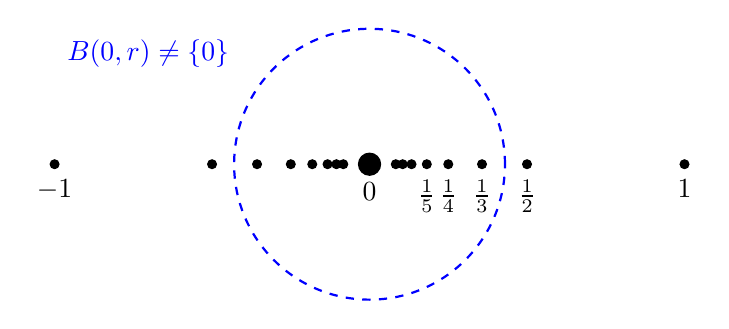
\begin{tikzpicture}[baseline={(0,0)}, scale=4]


% Define the coordinates of the points
\coordinate (x0) at (0,0);
\coordinate (x1) at (1,0);
\coordinate (x2) at (1/2,0);
\coordinate (x3) at (1/2.8,0);
\coordinate (x4) at (1/4,0);
\coordinate (x5) at (1/5.5,0);
\coordinate (x6) at (1/7.5,0);
\coordinate (x7) at (1/9.5,0);
\coordinate (x8) at (1/12,0);

% Define radii for the open balls around x and y (both equal to d(x, y) / 2)
\def\radius{0.43}  % Set r1 = r2 = d(x, y) / 2

% Draw the open balls as circles with dashed boundaries
\draw[blue, thick, dashed] (x0) circle (\radius) node[xshift=-80pt, yshift=40pt] {$B(0, r) \ne \{0\}$};
% \draw[red, thick, dashed] (y) circle (\radius) node[above right=4pt] {$B(y, \frac{d(x,y)}{2})$};

% Draw the points x and y
\filldraw[black] ($-1*(x1)$) circle (0.4pt) node[below, yshift=-2pt] {$-1$};
\filldraw[black] (x0) circle (1pt) node[below, yshift=-3pt] {$0$};
\filldraw[black] (x1) circle (0.4pt) node[below, yshift=-2pt] {$1$};
\filldraw[black] (x2) circle (0.4pt) node[below, yshift=-2pt] {$\frac12$};
\filldraw[black] ($-1*(x2)$) circle (0.4pt);
\filldraw[black] (x3) circle (0.4pt) node[below, yshift=-2pt] {$\frac13$};
\filldraw[black] ($-1*(x3)$) circle (0.4pt);
\filldraw[black] (x4) circle (0.4pt) node[below, yshift=-2pt] {$\frac14$};
\filldraw[black] ($-1*(x4)$) circle (0.4pt);
\filldraw[black] (x5) circle (0.4pt) node[below, yshift=-2pt] {$\frac15$};
\filldraw[black] ($-1*(x5)$) circle (0.4pt);
\filldraw[black] (x6) circle (0.4pt);
\filldraw[black] ($-1*(x6)$) circle (0.4pt);
\filldraw[black] (x7) circle (0.4pt);
\filldraw[black] ($-1*(x7)$) circle (0.4pt);
\filldraw[black] (x8) circle (0.4pt);
\filldraw[black] ($-1*(x8)$) circle (0.4pt);
%\node at (e) {$\cdots$};
%\node at (f) {$\cdots$};

% Draw the line connecting x and y
%\draw[thick, gray, {Latex}-{Latex}, shorten <= 2pt, shorten >= 2pt ] (x1) -- (x2) node[midway, above] {$1$};

\end{tikzpicture}
\end{document}
